\documentclass[a4paper]{article}

\usepackage[utf8]{inputenc}
\usepackage[T1]{fontenc}
\usepackage{textcomp}
\usepackage{listings}
\usepackage{lmodern}
\usepackage{amsfonts}
\usepackage{titling}
\usepackage{lipsum}
\usepackage[left=1in, right=1in, bottom=1in, top=1in]{geometry}
\usepackage{amsthm}
\usepackage{tcolorbox}
\usepackage{hyperref}
\usepackage{xcolor}
\usepackage{graphicx}
\usepackage{makeidx}
\usepackage{tikz}
\usepackage{cases}
\usepackage{apacite}
\usepackage{tkz-berge}
\usepackage{url}
\usepackage{tgtermes}
\usepackage{sectsty}
\usepackage{subcaption}
\usepackage{setspace}
\usepackage{float}
\usepackage{amsmath, amssymb}


% figure support
\usepackage{import}
\usepackage{xifthen}
\pdfminorversion=7
\usepackage{pdfpages}
\usepackage{transparent}
\usepackage{color}
\newcommand{\incfig}[2][1]{%
    \def\svgwidth{#1\columnwidth}
    \import{./figures/}{#2.pdf_tex}
}

%mathstyling
\theoremstyle{plain}
\newtheorem{thm}{Theorem}[section]
\newtheorem{lem}[thm]{Lemma}
\newtheorem{prop}[thm]{Proposition}
\newtheorem*{cor}{Corollary}

\theoremstyle{definition}
\newtheorem{defn}{Definition}[section]
\newtheorem{conj}{Conjecture}[section]
\newtheorem{exmp}{Example}[section]
\newtheorem{axiom}{Axiom}
\theoremstyle{remark}
\newtheorem*{rem}{Remark}
\newtheorem*{note}{Note}

\definecolor{darkgreen}{rgb}{0.0, 0.5, 0.0}

\pdfsuppresswarningpagegroup=1
\lstset{
tabsize = 4, %% set tab space width
showstringspaces = false, %% prevent space marking in strings, string is defined as the text that is generally printed directly to the console
numbers = left, %% display line numbers on the left
commentstyle = \color{darkgreen}, %% set comment color
keywordstyle = \color{blue}, %% set keyword color
stringstyle = \color{red}, %% set string color
rulecolor = \color{black}, %% set frame color to avoid being affected by text color
basicstyle = \small \ttfamily , %% set listing font and size
breaklines = true, %% enable line breaking
numberstyle = \tiny,
  frame=none,
  xleftmargin=2pt,
  stepnumber=1,
  belowcaptionskip=\bigskipamount,
  captionpos=b,
  escapeinside={*'}{'*},
  language=haskell,
  tabsize=2,
  emphstyle={\bf},
  showspaces=false,
  columns=flexible,
  showstringspaces=false,
  morecomment=[l]\%,
}
\begin{document}
	\begin{titlepage}
	\begin{center}
	\large
	University of Warwick \\
	Department of Computer Science \\
	\huge
	\vspace{50mm}
	\rule{\linewidth}{0.5pt} \\
	CS139 \\
	\vspace{5mm}
	\Large
	Web Development Technologies
	\rule{\linewidth}{0.5pt}
	\vspace{5mm}
	\begin{figure}[H]
	\centering
	
\includegraphics[width=0.4\textwidth]{crest.eps}
	\end{figure}
	\vspace{37mm}
	Cem Yilmaz \\
	\today
	\end{center}
	\end{titlepage}
	\newpage
	\tableofcontents
	\newpage
\section{HTML}
\subsection{Syntax}
HTML stands for HyperText Markup Language and is semantic. This means that it describes the structure of the document and not the content. It is intended to modify the appearance of HTML elements and can be in fact frustrating to use for page layouts.

A lot of HTML is done with the $<>$ brackets. For example,
\begin{lstlisting}[language = HTML , caption={Heading} , frame = trBL , firstnumber = last , escapeinside={(*@}{@*)}]
<h1>Welcome to CS139</h1>
\end{lstlisting}
This would set the header tag to the text "Welcome to CS139". For this module, we will be using JSFiddle, that is available online.
\subsubsection{Doctypes}
Every HTML documents should have a doctype definition on top. In particular, HTML5 uses
\begin{lstlisting}[language = HTML , caption={DOCTYPE} , frame = trBL , firstnumber = last , escapeinside={(*@}{@*)}]
<!DOCTYPE html>
\end{lstlisting}
It helps the browser to know what to expect.
\subsubsection{Example HTML5 Document}
\begin{lstlisting}[language = HTML , caption={Example Document} , frame = trBL , firstnumber = last , escapeinside={(*@}{@*)}]
<!DOCTYPE html>
<html>

	<head>
		<meta charset="UTF-8">
		<title>Title for Hello World </title> // Title that is seen at the top of the browser
	</head>
	<body>
		<h1>Hello world</h1> // Biggest header for the website
	</body>
</html>
\end{lstlisting}
\subsubsection{Head tag}
This tag is used by the browser, web-crawlers and bots. IT includes meta-tags required by these applications and includes location of supporting documents e.g. JavaScript and CSS.
\subsubsection{Text-encoding}
Familiar with ASCII, but that is only $128$ characters. In particular, UTF-8 has 107000 characters and is denoted with
\begin{lstlisting}[language = HTML , caption={Text-encoding} , frame = trBL , firstnumber = last , escapeinside={(*@}{@*)}]
<meta>
\end{lstlisting}
\subsubsection{Body tag}
This is the tag where main information goes into that the user gets to read. Its syntax is 
\begin{lstlisting}[language = HTML , caption={Body} , frame = trBL , firstnumber = last , escapeinside={(*@}{@*)}]
<body>
</body>
\end{lstlisting}
\subsubsection{Syntax}
\begin{lstlisting}[language = HTML , caption={Syntax} , frame = trBL , firstnumber = last , escapeinside={(*@}{@*)}]
<a href="google.com">Google search</a>
\end{lstlisting}
In the code above, $a$ is the element name. The hyperlink in href is called the \textit{Attribute}. The content is the \textit{Google search} text.
However, there are also empty tags e.g.
 \begin{lstlisting}[language = HTML , caption={Empty Tag} , frame = trBL , firstnumber = last , escapeinside={(*@}{@*)}]
<meta charset="utf-8">
\end{lstlisting}
\subsubsection{Nesting Definitions}
\begin{tcolorbox}[colback=black!3!white,colframe=black!60!white,title=\begin{defn}Child and parent \label{Child}\end{defn}]
A syntax is a child if and only if there exists a tag that is at a lower level than the upper tag.
\begin{lstlisting}[language = HTML , caption={Parent Child} , frame = trBL , firstnumber = last , escapeinside={(*@}{@*)}]
<body>
	<p>
	This is some text
	</p>
</body>
\end{lstlisting}
In particular, $<body>$ is the parent of $<p>$ and $<p>$ is the child of $<body>$.
\end{tcolorbox}
\begin{tcolorbox}[colback=black!3!white,colframe=black!60!white,title=\begin{defn}Sibling \label{Sibling}\end{defn}]
Sibling is when the tag is on the same level. For example,
\begin{lstlisting}[language = HTML , caption={Sibling} , frame = trBL , firstnumber = last , escapeinside={(*@}{@*)}]
<body>
	<p>
	This is some text
	</p>
	<p>
	Another text
	</p>
</body>
\end{lstlisting}
In here, the $p$ are siblings.
\end{tcolorbox}
Similarly, the term descendants would be group of tags of in comparison to a tag that is a parent of all.
\subsubsection{Lists}
There are 3 types of lists:
\begin{itemize}
	\item Ordered lists denoted with $<ol>$ and then listed items with $<li>$ 
	\item Unordered lists denoted with $<ul>$ and then listed items with $<li>$ 
	\item Description list would list terms and then list descriptions. In particular, the tags that are used are $<dl>$, $<dt>$ and $<dd>$ which are list, item and description respectively.You can also created nested list if you simply begin another list inside a list.
		
\end{itemize}
For example
\begin{lstlisting}[language = HTML , caption={Lists} , frame = trBL , firstnumber = last , escapeinside={(*@}{@*)}]
<ul>
	<li> shopping </li>
	<ol>
		<li> eggs </li>
		<li> bread </li>
	</ol>
	<li> cooking </li>
</ul>
\end{lstlisting}
\subsubsection{Hyperlinks}
\begin{flushleft}
Hyperlinks are listing websites to a specific piece of text. For example
\begin{lstlisting}[language = HTML , caption={Hyperlink} , frame = trBL , firstnumber = last , escapeinside={(*@}{@*)}]
<a href="www.google.com"> This is google hyperlink </a>
\end{lstlisting}
You can also hyperlink inside the website using ids. For example,
\begin{lstlisting}[language = HTML , caption={IDs} , frame = trBL , firstnumber = last , escapeinside={(*@}{@*)}]
<body>
<h1> Links </h1>
<p id = "#top">
	This is some paragraph text
</p>
<a href="#top"> Go to top </a>
\end{lstlisting}
\subsubsection{Images}
You can also include images with a singular tag that use the $src$ and $alt$ attributes.
For example,
\begin{lstlisting}[language = HTML , caption={Image embed} , frame = trBL , firstnumber = last , escapeinside={(*@}{@*)}]
<img src="http://warwick.ac.uk/logo.gif" alt="Warwick Logo" title="Warwick Logo" width=200 height=60 />
\end{lstlisting}
\subsubsection{Character entities}
\begin{lstlisting}[language = HTML , caption={Character entities} , frame = trBL , firstnumber = last , escapeinside={(*@}{@*)}]
&nbsp; //Nonbreakable space
&lt; //<
&gt; //>
&copy; //Copyright symbol
&trade; //Trademark symbol
\end{lstlisting}
\subsubsection{Break Line}
You can get a new line or break a line using the tag
\begin{lstlisting}[language = HTML , caption={Break} , frame = trBL , firstnumber = last , escapeinside={(*@}{@*)}]
<br>
\end{lstlisting}
\subsection{Semantic Mark-up}
Some semantics include but are not limited to
\begin{lstlisting}[language = HTML , caption={Semantics} , frame = trBL , firstnumber = last , escapeinside={(*@}{@*)}]
<abbr>
<cite>
<time>
<span>
<div>
\end{lstlisting}
That is, these do not change the looks but are important regardless. Usually, semantic mark-up refers to creating IDs on code to give meaning to piece of text and make it readable. In particular, the example in Hyperlinks with the ID is an example of a semantic mark-up.
\subsection{Validation}
You can make sure that your HTML is valid using a validation tool provided by W3C. The website is \link{http://validator.w3.org}
\subsection{Types of Style Sheet}
There are three different types of style sheet:
\begin{itemize}
	\item Author created style sheets
	\item User style sheets
	\item Browser style sheets
\end{itemize}
\subsection{Tables}
A lot of data in HTML conveys data in rows and columns, i.e., a table. 
\begin{lstlisting}[language = HTML , caption={Table} , frame = trBL , firstnumber = last , escapeinside={(*@}{@*)}]
<table>
	<tr>
		<td> The death of Marata </td>
		<td> Jacques-Louis David </td>
		<td> 1793 </td>
		<td> 162cm </td>
		<td> 128cm </td>
	</tr>
	<tr>
		<td> Burial at Ornans </td>
		<td> Gustave Courbet </td>
		<td> 1849 </td>
		<td> 314cm </td>
		<td> 663cm </td>
	</tr>
</table
\end{lstlisting}
In here, $</tr>$ stands for table row. $<td>$ stands for table data. Therefore cells in a row are declared by td, whereas rows are declared by tr. There is also $<th>$ which characterises table header. You can also add rowspan i.e.
\begin{lstlisting}[language = HTML , caption={Rowspan} , frame = trBL , firstnumber = last , escapeinside={(*@}{@*)}]
<table>
	<tr>
		<th> Artist </th>
		<th> Title </th>
		<th> Year </th>
	</tr>
	<tr>
		<td rowspan="3"> Jacques-Louis David </td>
		<td> The death of Marat </td>
		<td> 1793 </td>
	</tr>
	<tr>
		<td> The Intervention of Sabine Woman </td>
		<td> 1789 </td>
	</tr>
	<tr>
		<td> Napoleon Crossing the Alps </td>
		<td> 1800 </td>
	</tr>
</table>
\end{lstlisting}
Column span works in a similar fashion. Furthemore
\begin{lstlisting}[language = HTML , caption={Table Head and Footer} , frame = trBL , firstnumber = last , escapeinside={(*@}{@*)}]
<thead>
// Top of the table. It is always the top rows of a table.
</thead>
<tbody>
// Middle of the table. It is always inbetween header and foot.
<tbody>
<tfoot>
// Sets the last row of the table. This will always be at the bottom of the table.
</tfoot>
\end{lstlisting}
\subsection{Forms}
Sometimes we require to get data from the user, e.g. log-in page. It has the attributes:	
\begin{itemize}
	\item Action - the destination of the form data when submitted
	\item Method - the way in which the data is sent (GET or POST)
	\item Accept-charset - The charset accepted by the form
\end{itemize}
\begin{lstlisting}[language = HTML , caption={A basic form} , frame = trBL , firstnumber = last , escapeinside={(*@}{@*)}]
<form method="post" action="process">
	<fieldset>
		<legend> Details </legend>
		<p>
			<label> Title: </label>
			<input type="text" name="title" />
		</p>
		<p>
			<label> Country: </label>
			<select name="where">
				<option> Choose a country </option>
				<option> Canada </option>
				<option> Finland </option>
				<option> United States </option>
			</select>
		</p>
		<input type ="submit" />
	</fieldset>
</form>
\end{lstlisting}
\subsubsection{Attributes}
\begin{itemize}
	\item Type - the kind of input to accept
	\item Name - the name submitted to the server
	\item The value that you want the field to have
	\item Other attributes related to type...
\end{itemize}
\begin{lstlisting}[language = HTML , caption={Attributes} , frame = trBL , firstnumber = last , escapeinside={(*@}{@*)}]
<input type="text" name="city name" value="Warwick" >
<input type="text" name="uname" placeholder="what is your name" >
\end{lstlisting}
\subsubsection{Radio Buttons}
Radio buttons must have the same name in a group and allows you to select only a singular option
\begin{lstlisting}[language = HTML , caption={Radio Buttons} , frame = trBL , firstnumber = last , escapeinside={(*@}{@*)}]
<input type="radio" name="where" value="1">Coventry<br>
<input type="radio" name="where" value="2" checked>Warwick<br>
<input type="radio" name="where" value="3">Nottingham<br>
\end{lstlisting}
\subsubsection{Dropdown menus}
Dropdowns need $<option>$ elements with the $<select>$.
\begin{lstlisting}[language = HTML , caption={Dropdown menus} , frame = trBL , firstnumber = last , escapeinside={(*@}{@*)}]
<select name="choices">
	<option>First</option>
	<option selected>Second </option>
	<option> Third </option>
</select>	
\end{lstlisting}	
\subsubsection{Accessibility}
Sometimes we prefer the use of tables for data, not layout. In these cases, we use the caption element. This connect cells with a textual description in the header. You can also use "id" and "label for" to easen the accessability
\section{Introduction to Python/Flask}
\subsection{Flask and Python}
Flask is a server-side web micro-framework and it mainly uses Python as its scripting language. Its extensions provide further functionality. For example,
\begin{itemize}
	\item Dynamic HTML markup uses Jinja2
	\item Database access via SQLAchamy
	\item OThers such as Flask-WTF (forms) and Flask-Login (authentication)
\end{itemize}
It was released in 2010 and its version $2.0.2$ was released in October. Reddit, Linkedin, Netflix and Pinterest use it.
\subsection{General Architecture}
Python code is executed on a server and the output html is then sent to the client's browser.
\begin{figure}[H]
	\centering
	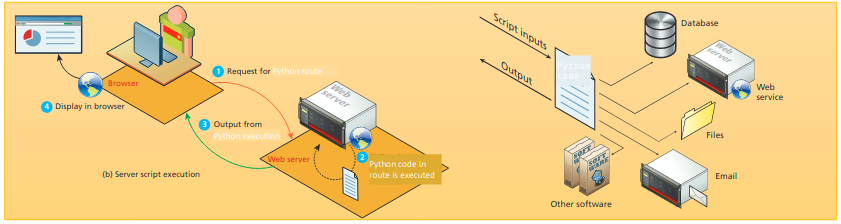
\includegraphics[width=0.8\textwidth]{architecture.png}
	\caption{Architecture of web server}
	\label{fig:architecture-png}
\end{figure}
\subsection{Flask and Python}
=Python is used to execute a web server and is written within a .py file. HTMl code is written in .html file. Python uses indentation for scoping without braces or semicolons. Comments use ectomorph simple or triple apostrophes e.g.
\begin{lstlisting}[language = Python , caption={Commenting} , frame = trBL , firstnumber = last , escapeinside={(*@}{@*)}]
# comment
''' comment '''
\end{lstlisting}
\subsection{Variable Naming}
Variables are duck=typed, i.e. dynamically and an integer. Variable names must begin with a letter or an underscore and cannot have spaces. Case sensitive value is not equal Value.
\subsection{Python Data Types}
Scalar types include
\begin{itemize}
	\item Integer
	\item Float
	\item Complex
	\item Boolean
	\item String
\end{itemize}
And compound types
\begin{itemize}
	\item Dictionary
	\item List and tuples
	\item Set
	\item Object
\end{itemize}
\subsection{Python Containers}
Python has $4$ containers types: Lists, Sets, Dictionaries and Tuples.
\begin{itemize}
	\item Lists are ordered and mutable, uses $[]$
	\item Sets are unordered and cannot have duplicates, uses $set\left(  \right) $ 
	\item Tuples are ordered and immutable, uses $(,)$ 
	\item Dictionaries are associative arraways - unordered values are references by their key, use $\{\}$
\end{itemize}
In particular, for examples, dictionaries can have "keys", e.g.
\begin{lstlisting}[language = Python , caption={Keys} , frame = trBL , firstnumber = last , escapeinside={(*@}{@*)}]
ages = {"Adam":27, "Dean":20, "Louise":30}
\end{lstlisting}
Then,
\begin{lstlisting}[language = Python , caption={Keys 2} , frame = trBL , firstnumber = last , escapeinside={(*@}{@*)}]
ages["Adam"] = 27
ages.update("Dean",20)
\end{lstlisting}
The key, which is their name, is linked to data which is their age.
\subsection{Python Functions}
You can define your own functions so that code is reusable. It is essentially creating methods. The code is
\begin{lstlisting}[language = Python , caption={Functions} , frame = trBL , firstnumber = last , escapeinside={(*@}{@*)}]
def <function name> (arg1, arg2...):
\end{lstlisting}
And these can return any object.
\subsection{Dealing with Forms}
Form values are submitted via a GET or POST method.
\begin{itemize}
	\item GET - encodes the parameters in the url, some of you have already discovered this
	\item POST - encodes form values in the message body.
\end{itemize}
Flask stores these values in the args(GET) or the form(POST) of the request object and we can pull out the values and do whatever we wish with them.
\subsection{Templates in Flask}
Web pages don't need to be created in Python and we can create HTML pages and render them from Python instead. An HTML page in Flask is called a Template and is stored in the Templates folder. IT is rendered using
\begin{lstlisting}[language = Python , caption={Template Render} , frame = trBL , firstnumber = last , escapeinside={(*@}{@*)}]
render_template(<pagename>)
\end{lstlisting}
And these templates have Jinja2 scripting. That is, these are not just HTML and they can be scripted and accept data from Python. For example,
\begin{itemize}
	\item Statements/scripts are written in $\{ \% \% \}$
	\item Expressions evaluated to the output are written in  $\{\{\} \} $ 
	\item Comments are written in $\{\# \#\} $
\end{itemize}
And this is useful because we can put shared elements into each page easily, i.e. headers, footers, menus etc. Furthermore, by keeping them in one place we can edit and have changes made in all pages.
\subsection{Object Oriented Python}
You can make python object oriented
\begin{lstlisting}[language = Python , caption={Object Oriented Python} , frame = trBL , firstnumber = last , escapeinside={(*@}{@*)}]
from flash impot Flask
app = Flash(__name__)

class Person :
	name = "unset"
	
	def get_name(self):
	return self.name;

	def set_name(self, new_name):
	self.name = new_name;

@app.route('/oop')
def oop():
	p = Person()
	p.set_name("Jane")
	return p.get_name()
\end{lstlisting}
Is an example of such, where we have a member variable called name and two functions get$\_$name and set$\_$name. To call methods on objects, we use the syntax
\begin{lstlisting}[language = Python , caption={Methods in objects} , frame = trBL , firstnumber = last , escapeinside={(*@}{@*)}]
object.method(<args>)
\end{lstlisting}
The $.$ is used regularly in Python to represent hierarchies (classes, modules etc.) If you want to import constructors, then you wrap the name of the constructor around double underscore. i.e. $\_\_\text{name}\_\_$.

Lastly, there is no such thing as private or protected in python. Instead, in variables, we name them with $\_\text{name}$ which is protected and $\_\_\text{name}$ which is a private variable. Lastly, inheritance can be done using 
\begin{lstlisting}[language = Python , caption={Inheritance} , frame = trBL , firstnumber = last , escapeinside={(*@}{@*)}]
class Admin(user):
\end{lstlisting}
This creates a subclass by using a class as a parameter to a class and you can also call parent class by
\begin{lstlisting}[language = Python , caption={Parent class} , frame = trBL , firstnumber = last , escapeinside={(*@}{@*)}]
super().method()
\end{lstlisting}
\section{Databases}
A web page can have the same structure: text,images,forms,tables,etc. even when the content is different. Web servers get the different data from a database. For databases, we use SQL. SQL stands for structured query language and is the language which you interact with Relational DataBase Management Systems (RDBMS). SQL is also a standard, however, database vendors extend their variants of SQL. It is possible to make a website with noSQL, and anther way to store is key-value pairs. No need for indexes and fast retrieval through other means e.g. hash-function. It is the same idea as dictionaries in Python. 
\begin{tcolorbox}[colback=black!3!white,colframe=black!60!white,title=\begin{defn}Database \label{Database}\end{defn}]
A data base is
\begin{itemize}
	\item A structure collection of data
	\item Arranged into tables
	\item Data may be queried
\end{itemize}
\end{tcolorbox}
In a to-do list, we would require to store
\begin{itemize}
	\item Users
	\item Lists
	\item ListItems
\end{itemize}
And each of these will be stored in tables.
\subsection{Management}
Databases often require permissions to access the data, such as users, passwords, access rights and etc. Managing the database is a complex process and is beyond the scope of this web-dev module. For simplicity we will use SQL called sqlite3. 
\subsection{Database table}
A table is placed to store data of the same type. You decide on the columns in the table, and these usually represent the data which you will store. The rows of the table are the data that is entered. A table has a fixed number of columns, but may have an unlimited number of rows. You can think of it like a spreadsheet. 
\\ For example
\begin{tcolorbox}[colback=black!3!white,colframe=black!60!white,title=\begin{exmp}Creating users table \label{Creating users table}\end{exmp}]
        
\begin{table}[H]
	\centering
	\caption{Example Database}
	\label{tab:database}
	\begin{tabular}{|c|c|}
		\hline
	Name &  Datatype \\
	\hline
	email & varchar(50) \\
	nickname & varchar(20) \\
	biography & text \\
	password* & varchar(25)\\
	\hline
	\end{tabular}
\end{table}
\end{tcolorbox}
Note that it isn't the best way to store password but it is sufficient for current purposes
\subsection{Relating data}
For example, in an online forum, Users require to write leading to posts. Posts are a part of threads which belong to forums. Sites have many forums. Forum features must be view all posts by a user and get all threads in a forum. It should be able to find all users who posted in forum A, but not forum B on Tuesday.
\subsection{SQL Datatypes}
The SQL datatypes are
\begin{itemize}
	\item integer - whole numbers
	\item real - decimal numbers
	\item text
\item blob - binary data
\item varchar(length) - fixed length test
	\item datetime - date and time
	\item date
\end{itemize}
\subsection{Unique Rows}
We designate a column in a table as the primary key of the database. It requires that each column is unique in that row. Most databases have an auto increment from $1$. Designating a column as an integer primary key creates an auto incrementing value in SQLite. 
\subsection{SQL Operations}
You can test SQL operations using the website https://sqliteonline.com
The basic operations we are going to consider are:
\subsubsection{Creating a table}
\begin{lstlisting}[language = SPARQL , caption={Creating table} , frame = trBL , firstnumber = last , escapeinside={(*@}{@*)}]
CREATE TABLE <table name>(<column 1 datatype>, ...<columnN datatype>);
\end{lstlisting}
\begin{tcolorbox}[colback=black!3!white,colframe=black!60!white,title=\begin{exmp}Creating users table \label{Creating users table}\end{exmp}]
\begin{lstlisting}[language = SPARQL , caption={Creating Users Tabl} , frame = trBL , firstnumber = last , escapeinside={(*@}{@*)}]
CREATE TABLE users(email varchar(50), nickname varchar(20), biography text, password varchar(25));
\end{lstlisting}        

And if we want to have an auto incrementing primary key for our example
\begin{lstlisting}[language = SPARQL , caption={Primary key} , frame = trBL , firstnumber = last , escapeinside={(*@}{@*)}]
CREATE TABLE users(id integer primary key, email varchar(50), nickname varchar(20), biography text, password varchar(25));
\end{lstlisting}
\end{tcolorbox}
\subsubsection{Inserting data}
To insert data into the table we use the insert statement as follows:
\begin{lstlisting}[language = SPARQL , caption={Inserting data} , frame = trBL , firstnumber = last , escapeinside={(*@}{@*)}]
INSERT INTO <table name> VALUES(value1, ..., valueN);

\end{lstlisting}
\begin{tcolorbox}[colback=black!3!white,colframe=black!60!white,title=\begin{exmp}Inserting data to table with ID \label{Inserting data to table with ID}\end{exmp}]
        \begin{lstlisting}[language = SPARQL , caption={Inserting data to table with ID} , frame = trBL , firstnumber = last , escapeinside={(*@}{@*)}]
        INSERT INTO users VALUES(NULL, "apc@dcs.warwick.ac.uk", "Adam", "Lecturer..", "123asdh2qd");
        \end{lstlisting}
\end{tcolorbox}
\subsubsection{Updating data}
We can update existing database records using the UPDATE function as seen below:
\begin{lstlisting}[language = SPARQL , caption={Updating data} , frame = trBL , firstnumber = last , escapeinside={(*@}{@*)}]
UPDATE <table name> SET <column> = <new value> ... ;
\end{lstlisting}
But if we require to run this we update the column for all rows in the database. Sometimes we need to select the right row
\begin{lstlisting}[language = SPARQL , caption={Selecting the right row to update} , frame = trBL , firstnumber = last , escapeinside={(*@}{@*)}]
UPDATE <table name> SET <column> = <new value>, ... WHERE <column> = <value>;
\end{lstlisting}
\begin{tcolorbox}[colback=black!3!white,colframe=black!60!white,title=\begin{exmp}Editing existing values \label{Editing existing values}\end{exmp}]
        \begin{lstlisting}[language = SPARQL , caption={Updating users} , frame = trBL , firstnumber = last , escapeinside={(*@}{@*)}]
        UPDATE users SET password = "12345", nickname = "andrew" WHERE id = 2
        \end{lstlisting}
\end{tcolorbox}
\subsubsection{Deleting data}
The delete command is defined as follows:
\begin{lstlisting}[language = SPARQL , caption={Deleting data} , frame = trBL , firstnumber = last , escapeinside={(*@}{@*)}]
DELETE FROM <table name> WHERE <column> = <value>
\end{lstlisting}
Note that if you forget the WHERE close, all rows are deleted.
\begin{tcolorbox}[colback=black!3!white,colframe=black!60!white,title=\begin{exmp}Users deletion \label{Users deletion}\end{exmp}]
        \begin{lstlisting}[language = SPARQL , caption={Deleting data from USERS} , frame = trBL , firstnumber = last , escapeinside={(*@}{@*)}]
        DELETE FROM users WHERE id = 3
        \end{lstlisting}
	This will delete the rows with $\text{id} = 3$
\end{tcolorbox}
\subsubsection{Selecting data}
We can limit our queries by adding WHERE clause.
\begin{lstlisting}[language = SPARQL , caption={Selecting data} , frame = trBL , firstnumber = last , escapeinside={(*@}{@*)}]
SELECT email from users WHERE ("newsletter"="true");
\end{lstlisting}
i.e., this will create a table with only email column with people whose newsletter is true.
\subsubsection{Joining tables}
We can join tables by extracting column data from any table that we desire. In particular,
\begin{lstlisting}[language = SPARQL , caption={Joining tables} , frame = trBL , firstnumber = last , escapeinside={(*@}{@*)}]
SELECT * FROM posts WHERE ("user_id" = 1)
\end{lstlisting}
That is, we could query them from multiple sources.
\subsection{Flask - SQLAlchemy}
\subsubsection{Advantages and Disadvantages of SQLite3}
\begin{table}[H]
	\centering
	\caption{Advantages and Disadvantages}
	\label{tab:andd}
	\begin{tabular}{|c|c|}
	 \hline
	 Advantages & Disadvantages \\ \hline
	 Public domain (free and open source) & Lack of support \\
	 Easy to install & Not fully ACID compliant \\
	 Easy to work with & Does not support concurrent writes \\
	 \hline
	\end{tabular}
\end{table}
\subsubsection{Connecting to a SQLite database}
Connectiong to a SQLite database is simple and requires no usernames, passwords, hostnames or ports to deal with. \\
A connection to the database from the Flask 'app' can be made using
\begin{lstlisting}[language = Python , caption={Importing SQLite} , frame = trBL , firstnumber = last , escapeinside={(*@}{@*)}]
from flask_sqlalchemy import SQLAlchemy
db = SQLAlchemy()
db.init_app(app)
\end{lstlisting}
You may not run code by calling methods on newly created connection stored in $db$. \\
However, the 'app' needs to be configured first with some SQLAlchemy values, i.e.
\begin{lstlisting}[language = Python , caption={Configuration} , frame = trBL , firstnumber = last , escapeinside={(*@}{@*)}]
app.config['SQLALCHEMY_TRACK_MODIFICATIONS'] = False
app.config['SQLALCHEMY_DATABASE_URI'] = f'sqlite:///{db_abs_location}'
\end{lstlisting}
And the location of the database must be an absolute filename:
\begin{lstlisting}[language = Python , caption={Location of DB} , frame = trBL , firstnumber = last , escapeinside={(*@}{@*)}]
import os
basedir = os.path.abspath(os.path.dirname(__file__))
db_abs_location = os.path.join(basedir, 'sqlalchemy.sqlite')
\end{lstlisting}
\subsubsection{Populating the database}
The database requires a schema and some default data. For this, we use a Python file containing the schema and it can be found in Moodle. In particular, for the schema on forums in moodle we have:
\begin{figure}[H]
    \centering
    \incfig{schema}
    \caption{schema}
    \label{fig:schema}
\end{figure}
\subsubsection{Differences between SQL and SQLAlchemy}
We use $String(n)$ instead of $varchar(n)$. Furthermore, when we create a table, we define it using the $Model$ class. 
\begin{tcolorbox}[colback=black!3!white,colframe=black!60!white,title=\begin{exmp}Table using SQLAlchemy \label{Table using SQLAlchemy}\end{exmp}]
        \begin{lstlisting}[language = Python , caption={Table using SQLAlchemy} , frame = trBL , firstnumber = last , escapeinside={(*@}{@*)}]
        class Users(db.Model):
		__tablename__='users'
		id = db.Column(db.Integer, primary_key = True)
		email = db.Column(db.String(50))
		nickname = db.Column(db.String(20))
		biography = db.Column(db.Text())
		password_hash = db.Column(db.String(25))
        \end{lstlisting}
\end{tcolorbox}
And to actually create these tables, we then need to run the code
\begin{lstlisting}[language = Python , caption={Table creation} , frame = trBL , firstnumber = last , escapeinside={(*@}{@*)}]
@app.route('/create')
def create_db():
	db.create_all()
	return "tables created"
\end{lstlisting}
Alternatively,
\begin{lstlisting}[language = Python , caption={Table creation alternative} , frame = trBL , firstnumber = last , escapeinside={(*@}{@*)}]
with app.app_context():
	db.create_all()
\end{lstlisting}
\subsubsection{Executing Queries}
Once a connection is created you can query the database and there are two ways to submit a query with SQLAlchemy:
\begin{itemize}
	\item $db.session$ which is suitable for result-less queries (add, delete, update)
	\item $Model.query$ which begins a query on a Table(Model). This is the same as SELECT.
\end{itemize}
\subsubsection{Database Example (Adding data, linking)}
A database example can be found in moodle can be executed using
\begin{lstlisting}[language = Python , caption={Executing example} , frame = trBL , firstnumber = last , escapeinside={(*@}{@*)}]
from forumschema import db, Users, Forums, Threads, Posts, dbinit

db.init_app(app)

with app.app_context():
	db.create_all()
	dbinit()
\end{lstlisting}
In particular, the file in case missing is as following:
\begin{lstlisting}[language = Python , caption={File} , frame = trBL , firstnumber = last , escapeinside={(*@}{@*)}]
# import SQLAlchemy
from flask_sqlalchemy import SQLAlchemy

# create the database interface
db = SQLAlchemy()

# a model of a forum for the database
class Forum(db.Model):
    __tablename__='forums'
    id = db.Column(db.Integer, primary_key=True)
    name = db.Column(db.Text())
    headline = db.Column(db.Text())

    def __init__(self, name, headline):
        self.name=name
        self.headline=headline


# a model of a forum for the database
class Thread(db.Model):
    __tablename__='threads'
    id = db.Column(db.Integer, primary_key=True)
    title = db.Column(db.Text())
    message = db.Column(db.Text())
    created_at = db.Column(db.DateTime())
    forum_id = db.Column(db.Integer(), db.ForeignKey('forums.id') )

    def __init__(self, title, message, created_at, forum_id):
        self.title=title
        self.message=message
        self.created_at=created_at
        self.forum_id=forum_id



from datetime import datetime
import time

def dbinit():
    db.session.add(Forum("Lab Sessions", "Discuss Lab Sessions here"))
    db.session.add(Forum("Lectures", "Discuss lectures here"))
    db.session.add(Forum("General", "Discuss anything else here"))

    posttime = datetime(2022,2,4,18,0)
    
    db.session.add(Thread("Lab 2 help", "Anybody good at CSS?",posttime,1))
    db.session.add(Thread("Can you smell doughnuts?", "I think so",posttime,1))
    db.session.add(Thread("Python win", "This is true",posttime,1))

    time.sleep(1)
    db.session.add(Thread("Great lecture", "Best. Lecture. Ever!", datetime.now(),2))
    time.sleep(1)
    db.session.add(Thread("I LOVE CS139", "It is so good", datetime.now(),2))

    db.session.commit()
\end{lstlisting}
\subsubsection{Add data to the forum}
The index pages requires a number of forums from the forum table, and to write a query to fetch everything from the forums we write
\begin{lstlisting}[language = Python , caption={Fetch All} , frame = trBL , firstnumber = last , escapeinside={(*@}{@*)}]
SELECT * FROM FORUMS;
\end{lstlisting}
However in SQLAlchemy instead we write this as
\begin{lstlisting}[language = Python , caption={SQLAlchemy Fetch All} , frame = trBL , firstnumber = last , escapeinside={(*@}{@*)}]
rows = Forums.query.all()
\end{lstlisting}
And when a set of results is returned, each row is a data object. The columns of the row can be accessed by name. In particular,
\begin{lstlisting}[language = Python , caption={Access of data} , frame = trBL , firstnumber = last , escapeinside={(*@}{@*)}]
forums = Forums.query.all()
s = ""
for entry in forums:
	s += f"{entry.name}<br>"
\end{lstlisting}
\subsubsection{Serialisation in Python}
Serialisation enables data to be moved in and out of variables, including objects. This is useful if you want to store complex data in your database or a file. Serialisation in Python comes in two forms:
\begin{itemize}
	\item import pickle
	\item import json
\end{itemize}
It is useful for transferring the data.
\subsection{GET request and response}
Request a resource e.g. a file \\
Response has $2$ sections
\begin{enumerate}
	\item A header containing the status of the request
	\item An optional body containing the response to the request
\end{enumerate}
\subsubsection{Response Codes}
The response codes for the requests are:
\begin{itemize}
	\item $2\#\#$ coes are for successful responses,
	\item $3\#\#$ are for redirection-related responses,
	\item $4\#\#$ are for client errors,
	\item $5\#\#$ are for server errors.
\end{itemize}
where hashtags are numbers.
However, it is particular important to remember the following response codes:
\begin{itemize}
	\item $200$ - OK Success
	\item $301$ - Moved Permanently 
	\item $404$ - Not found
	\item - Internal server error
\end{itemize}
\section{Internet Protocols}
Computers need to communicate in the same language and TCP/IP exists in every operating system and this allows for such communication. However, be aware that networking is an entirely separate discipline and web dev just needs an awareness of these protocols - it's the curtain between your web-app and the rest of the world. 
\subsection{Layers of protocol}	
\begin{enumerate}
	\item HTTP: Hypertext Transfer Protocol - used for web communication
	\item FTP: File Transfer Protocol - used for transferring files between computers
	\item POP/IMAP/SMTP - Email-related protocols for transferring and storing mail
	\item DNS: Domain Name System - protocol used for resolving domain names to IP addresses
\end{enumerate}
\subsection{IP Address}
\subsubsection{IPv4}

IP addresses needed by every computer on the internet. For example, IPv4 uses $4\times 8-$bit numbers.
\begin{itemize}
	\item 127.0.0.1 - localhost
	\item 192.168.*.* and 10.0.*.* are for private networks
	\item There are other reserved addresses and ranges
\end{itemize}
All IPv4 numbers, i.e., $256^{4}$ addresses are gone.
\subsubsection{IPv6}
We now use IPV6, for which uses $8\times 16-$ bit numbers which results in $340$ undecillion addressses. It looks like, for example:
$2001:0db8:0000:0000:0000:ff00:0042:8329$
\subsection{Network Address Translation (NAT)}
A device connects to a router's internal address and then router opens a port and connects to the external resource. Data received is then passed through the router to the originating device
\subsection{Domain Name System (DNS)}
Domain name system servers are a 'contacts list' for internet servers. It translates human readable name to an IP address and it is a hierarchic distribution naming system for resources on the internet.
\begin{tcolorbox}[colback=black!3!white,colframe=black!60!white,title=\begin{exmp}Domain Namespace \label{Domain Namespace}\end{exmp}]
        
                \begin{align}
       \underbrace{\text{server1}}_{\text{Fourth-level domain}}.\overbrace{\text{www}}^{\text{Third-level domain}}.\underbrace{\text{funwebdev}}_{\text{Second-level domain (SLD)}}.\overbrace{\text{com}}^{\text{Top-level Domain (TLD)}}
                \end{align}
\end{tcolorbox}
That is, it is a tree of domain spaces. Zero or more resources records exist at each node of tree and the root zone is the TLD, and is controlled by the Assigned Numbers Authority. Registrars assigned domain names beneath the TLD and check with interNIC, the canonical source for the domain names. 
\subsection{Resolving a domain name}
A network host is primed with the addresses of the root name server. The client sends a query to a root name server and query the top level domain server for the authoritative nameserver for the domain. Last step repeats for each additional subdomain request. 
\begin{tcolorbox}[colback=black!3!white,colframe=black!60!white,title=\begin{exmp}Wikipedia \label{Wikipedia}\end{exmp}]
        The DNS recurses asks for the IP address of the DNS $www.wikipedia.org$. To do so, it connects to the root nameserver. The rootname server redirects to the .org nameserver. The .org nameservers then redireects to wikipedia as required.
\end{tcolorbox}
\subsection{Domain Name Caching}
Not every request from every web user is sent to root nameservers as this would take a massive load. In partice, NS record caching is used to overcome this throughout internet. For example, your ISP will have the IPs of common domain names like google.com and bbc.co.uk to avoid overload. Time to live (TTL) dictates how long a DNS record should remain valid.
\subsection{Uniform Resource Locators}
\begin{align}
	\overbrace{\text{http}}^{\text{protocol}}:\slash\slash\underbrace{\text{www.funwebdev.com}}_{\text{Domain}}\slash\overbrace{\text{index.php}}^{\text{path}}?\underbrace{\text{page=17}}_{\text{Query String}}\# \overbrace{\text{article}}^{\text{fragment}}
\end{align}
\subsection{IP Address, Domain Name and URL}
DNS is case insensitive and so the URL is also case insensitive. IP Address can be used for the domain. Ports, on the other hand, can also be given. We add : (colon) in an integer to specificy the port i.e., \\
\begin{align*}
	\text{http:\slash\slash www.funwebdev.com:5000\slash index.php}
\end{align*}
\subsection{Path}
When making an HTTP or FTP request, it is a file that you are requesting and $\slash$ is the root folder on that server, just like your local file system. If a file is not specified, then webserver will choose a file for you, by default this is usually the $index.html$. The path IS case sensitive.
\subsection{Query string}
This provides information to the web servers and is a sequence of key-value pairs after a question mark, separated by ampersands. For example
\begin{table}[H]
	\centering
	\caption{Data}
	\label{tab:data}
	\begin{tabular}{|c|c|}
		\hline
	Key & Value\\
	\hline
	page & $12$ \\
	colour & red\\
	\hline
	\end{tabular}
\end{table}
	Would be represented by
	\begin{align*}
		\text{...index.php?page=12\&colour=red}
	\end{align*}
	We can access data that is passed via get or post methods through the request object in Flask and conventionally we use
	\begin{itemize}
		\item GET when requesting data : $\slash$forum?page=1
		\item POST when sending data: forms
	\end{itemize}
	\subsection{Fragment}
	Fragment is a method of requesting a portion of a page and used by the HTML anchor tag $<a>$, for example
	\begin{align*}
		\text{...index.php\#article}
	\end{align*}
	\subsection{Hypertext Transfer Protocol}
	HTTP is an application protocol for hypermedia information systems and it standardises the request-response message. Its development coordinated by Internet Engineering Task Force (IETF) and World Wide Web Consortium (W3C). Version HTTP$\slash 1.1$ is in common use. HTTP$\slash2$ published in $2015$. HTTP$\slash3$ drafted in $2020$.
	\subsection{Web browser}
	The resource provided by the web server will be raw data, usually text or encoded binary. A web browser interprets the data and displays it in a recognised form:
	\begin{itemize}
		\item It is converting HTML page data and rendering it as a readable web page
		\item Each browser has different method of doing this, but they 'loosely' conform to most of the standard
	\end{itemize}
	Local browser caching also exists, for which reduces the amount of data being transferred to the root nameservers. These also contain additional features which include, but are not limited to, phishing detection, URL autocomplete etc.
	\subsection{Stateless-ness}
	HTTP is a stateless protocol and in a local process, the computer knows about the current state of memory and instructions. In a web process, the server treats every request as a completely new request with no historical state. Transfer the next 'state' back to the end user for their use. For this, we have 3 solutions:
	\begin{itemize}
		\item Query String
			\begin{itemize}
				\item URL Path Rewriting
			\end{itemize}
		\item Cookies
		\item Sessions
	\end{itemize}
	\subsubsection{Query String}
	Because query string was mentioned earlier, we will focus on the URL path in here instead. Dynamic URLs i.e., query strings are pretty essential part of web application development. Static URLs, on the other hand:
	\begin{itemize}
		\item The appearance of search terms within the URL does seem to improve its relative position in SEO
		\item Another benefit to static URLs is that users tend to prefer them
		\item Can use URL rewriting to make static URLs be dynamic
	\end{itemize}
	\subsubsection{Cookies}
	Cookies is data unique to the client that is created by the server. The server sends a cookie back to the client when the first request is made and the client incorporates that cookie in subsequence requests. The client incorporates that cookie in subsequence requests. These usually expire when the browser session ends and are restricted to the domain e.g., mysite.com. In flask:\\
	\begin{itemize}
		\item The server-side (Flask) sets the cookie in the response
		\item make_response to create the response
		\item set_cookie to add the cookie to the response header
	\end{itemize}
\begin{lstlisting}[language = Python , caption={Cookies} , frame = trBL , firstnumber = last , escapeinside={(*@}{@*)}]
@app.route('/setcookie')
def methoud():
	username=request.args.get('name')
	message=request.args.get('mesg')

	resp = make_response(render_template_string("{{message}}", \
		message=f'Responding to "{message}" sent by "{username}"'))
	
	resp.set_cookie('usercookie', username, max_age=60)

	return resp
\end{lstlisting}
This cookie grabs the name and message from the query string and generates a response and inputs the defined message. \\
For checking cookies we do a server-side access on request.cookies for data it set last time. In particular,
\begin{lstlisting}[language = Python , caption={Checking Cookies} , frame = trBL , firstnumber = last , escapeinside={(*@}{@*)}]
def checkcookie():
	name = request.cookies.get('usercookie')
	if name is None:
		name = 'not found'
	return f'<h1>usercookie: {name}</h1>'
\end{lstlisting}
A demo of this exists in the CS139 moodle page.
\subsubsection{Sessions}
Sessions store data just for the time that a user is active in the website. This data is synchronised securely with the server and server can store the session information with other distributed methods e.g. Memcache. It is especially useful for user authentication: login and logout.\\
In flask, we use session object to save information for the session. In particular,
\begin{lstlisting}[language = Python , caption={Session Flask} , frame = trBL , firstnumber = last , escapeinside={(*@}{@*)}]
from flask import Flask, request, redirect, render_template, session
app = Flask(__name__)
app.secret_key = 'any string you want'

@app.route('/')
def method():
	if 'usename' in session:
		username = session('username')
		return f'Logged in as {username}<br>'+\
			'<b><a href="/logout">Logout</a>'

	return 'You need to log in <br>'+\
		'<b><a href="/login">Login</a>'
\end{lstlisting}
We can store data in a session using a dictionary and put in values by writing
\begin{lstlisting}[language = Python , caption={Session object} , frame = trBL , firstnumber = last , escapeinside={(*@}{@*)}]
session['key'] = value
\end{lstlisting}
And retrieve them with
\begin{lstlisting}[language = Python , caption={Session object retrieval} , frame = trBL , firstnumber = last , escapeinside={(*@}{@*)}]
value = session['key']
\end{lstlisting}
Python can test dictionary membership with in $<value>$ in session. So for example, we could do
\begin{lstlisting}[language = Python , caption={Example} , frame = trBL , firstnumber = last , escapeinside={(*@}{@*)}]
if 'user_id' not in session:
	return redirect('index');
\end{lstlisting}
Which would test for a userid key set in the session. Finally, to close the session we can simply pop() the individual session keys. Or we can clear() all the keys. In fact, flask provides a way for a session to end when the browser closes also by using
\begin{lstlisting}[language = Python , caption={Flask browser close session} , frame = trBL , firstnumber = last , escapeinside={(*@}{@*)}]
session.permanent = False
\end{lstlisting}
And to summarise:
\begin{itemize}
	\item To create a session in Flask add entries in the session object
	\item Create a session variable in the object e.g.
	\begin{lstlisting}[language = Python , caption={Creating session variable} , frame = trBL , firstnumber = last , escapeinside={(*@}{@*)}]
	session['username']='Adam'
	\end{lstlisting}
\item Release the session variable using pop() e.g.
	\begin{lstlisting}[language = Python , caption={Release session} , frame = trBL , firstnumber = last , escapeinside={(*@}{@*)}]
	session.pop('username', None)
	\end{lstlisting}
\item and to finally set the secret key:
	\begin{lstlisting}[language = Python , caption={Secret key} , frame = trBL , firstnumber = last , escapeinside={(*@}{@*)}]
	app.secret_key = 'any string you want'
	\end{lstlisting}

\end{itemize}

\section{CSS}
\subsection{Cascade}
Styles are applied in the following order:
\begin{itemize}
	\item Browser default
	\item External style sheet
	\item Internal style sheet
	\item Inline styling
\end{itemize}
However, in terms of inheritance, only some properties are inherited because it is complicated.
\subsection{Syntax}
The commands modify the styling of your HTML, and for instance,
\begin{lstlisting}[language = CSS , caption={CSS example} , frame = trBL , firstnumber = last , escapeinside={(*@}{@*)}]
h1 {
	color: blue;
	font-size: 12px;
}
\end{lstlisting}
\subsection{Selectors}
Notice how all $<h1> $ tags will be modified the same way. A class selector can be used to modify just some HTML elements: we use fullstops to denote a class. An ID selector can e used to modify unique HTML element as well. These are done by denoting classes and then modifying the style of these classes
\begin{lstlisting}[language = CSS , caption={Class} , frame = trBL , firstnumber = last , escapeinside={(*@}{@*)}]

\end{lstlisting}
\begin{lstlisting}[language = CSS , caption={ID} , frame = trBL , firstnumber = last , escapeinside={(*@}{@*)}]

\end{lstlisting}
\begin{lstlisting}[language = CSS , caption={} , frame = trBL , firstnumber = last , escapeinside={(*@}{@*)}]
\end{lstlisting}
More information can be found in https://www.w3schools.com/cssref/css_selectors.asp
\subsection{Pseudo-elements}
A pseudo-selector targets a particular state or relationship e.g. the $<a>$ tag. An example of pseudo-element is the following:
\begin{lstlisting}[language = HTML , caption={Pseudo selector} , frame = trBL , firstnumber = last , escapeinside={(*@}{@*)}]
<style>
p::selection {background-color:green;}
</style>
\end{lstlisting}
\subsection{Box Model}
All elements on a page are boxes. They all have width and height. 
Block level elements start and end with a new line. For example, $<h1>$, $<p>$, $<table>$ are all block level elements. That is, they would become separate lines. \\
There are also inline elements, that is, boxes which are not in separate lines. Examples include $<a>$, $<img>$ etc. 
\section{Security}
\subsection{Login}
To prevent unwanted access to a web page, we could add something along the lines of
\begin{lstlisting}[language = Python , caption={Login} , frame = trBL , firstnumber = last , escapeinside={(*@}{@*)}]
from flask_login import login_required 

@login_required #denotes that login is required for a webpage
login_manager.login_view="login" #where to redirect if not logged in
\end{lstlisting}
\subsection{Sanitising Query Strings}
Sometimes query strings are not as expected, that is:
\begin{itemize}
	\item Parameter may not exist or,
	\item Parameter does not contain a value or,
	\item Query string parameter value isn't correct type or is out of range or,
	\item Value is required for a database lookup but the provided value does not exist in the db
\end{itemize}
These are expected errors and require error checking.
\subsection{HTTPS}
HTTPS was used until quite recently when it changed in 2011. All requests and all responses used plain text by default and then HTTPS was introduced. It is a protocol for secure communication over a network with an extra protocol on HTTP called SSL/TLS protocol. In other words, information is not encrypted. \\
A client and server build a TCP (point-to-point) connection. The client sends a number of specifications to the server:
\begin{itemize}
	\item What version of SSL/TLS is being executed
	\item Which cipher suites it wants to use
	\item Which compression method to use
\end{itemize}
The server selects the highest SSL/TLS version supported by both, picks a cipher suite and optionally a compression method. The server sends its certification and it must either be trusted explicitly OR a party that the client trusts. After verifying the server's certification, an asymmetric key is exchanged. Both client and server setup a key for symmetric encryption and the client tells the server that all communication must be encrypted. \\
The server verifies the MAC address (used for authentication) is correct and the message can be correctly decrypted. Handshake is then complete. 
\subsubsection{Disadvantages}
Speed - setting up the encrypted connections can be expensive. Furthermore, some servers have dedicated encryption hardware to speed up the encryption operations. 
\subsection{The role of certificates}
Creating a secure connection with a server would require knowing its public key. However it would be impractical to store the public keys for every server in the internet. The solution is certificate authorities (CA). In other words, a third party would be required to store all public keys, in order to ensure that the source is legitimate. The issue is, however, that anyone can become a CA and you may be the only one that trusts it. \\
HTTPS should be used whenever sensitive data is being passed between client and server. Was used solely for e-commerce but now is being used widely.
\subsection{Man-in-the-middle attacks}
Data was sent via HTTP may be subject to man in the middle attack. A man in the middle attack consists of the following stages:
\begin{itemize}
	\item Alice and Bob would like to have a conversation with Michael helping them
	\item Bob sends his key to Michael and Michael responds to Alice with his own key
	\item Alice encrypts her message using Michael's key, believing it to be Bob's. Michael can read the message and forward a modified message using Bob's key.
\end{itemize}
\subsection{SQL Injection}
Even with encryption connections, nefarious instructions can still be transmitted. More specifically, snippets of SQL are sent via user submitted fields to attempt get the server to execute the rogue SQL. For example,
\begin{lstlisting}[language = SQL , caption={SQL Injection} , frame = trBL , firstnumber = last , escapeinside={(*@}{@*)}]
qry = f"SELECT * FROM employees WHERE name = '{username}';"
\end{lstlisting}
You would not want to have similar code in your TODO list applications! \\
Now we consider a username of ' or '1'='1
This username would cause your program to create this string query:
\begin{lstlisting}[language = SQL , caption={SQL Injection Name} , frame = trBL , firstnumber = last , escapeinside={(*@}{@*)}]
SELECT * FROM employees WHERE '' or '1'='1'
\end{lstlisting}
And the output from this would be all employees in the database.
\subsubsection{Solution: Escape SQL Characters}
You could evaluate and escape all user input. For example, username = username.replace("",""") but replacing characters is really bad as there are too many special characters and scenarios to consider. In other words, one forgotten parameter is then a vulnerability.
\subsubsection{Solution: Parameterised statements}
The query string is not built at runtime, it is written with placeholder values to which variables are bound. Placeholders are restricted by type, and thus invalid if an incorrect strings is passed to them. Values are bound to placeholders.
\subsection{Database permissions}
Restrict access to system tables, we need to limit exposure of tables on a per-user basis. For RDBMS with permissions (not SQLite). 
\subsection{Session Hijacking}
There are a number of ways that an attacker can hijack a user session which include
\begin{itemize}
	\item Session sniffing - All unencrypted network traffic is vulnerable to network traffic. Cookies which store a user's data could be reconstructed and then used by an attacker to impersonate the user
	\item Session fixation - Attacker sets the user's session ID to one known to him. Then waits for the user to log on.
\end{itemize}
\subsection{Cross Site Scripting (XSS)}
XSS allows users to inject client side script into webpages. It is accounted for about $84\%$ of all security vulnerabilities documented by Symantec in 2007. Non-persistent data provided by client is used immediately by server-side scripts without proper sanitisation, thus content is uploaded is included back into the pages. It is essentially like crafting a GET request. For example,
\begin{lstlisting}[language = Python , caption={XSS} , frame = trBL , firstnumber = last , escapeinside={(*@}{@*)}]
username = request.args.get('name')
hello_html = f"<p>Hi {username}</p>" 
\end{lstlisting}
This is an awful script because the input is no filtered and the output is not escaped. \\
Because the remote script is run on your page in the browser, it has access to everything. It can steal cookies for session hijacking and change the HTML in the page, e.g. add forms for payments. \\
To deliver XSS attack, simply the user a link, with the <a href set to the crafted URL. Content is inserted into pages, appearing as if from the correct site.
\subsubsection{Solution: Filtering the input using jinja2 markup}
\begin{lstlisting}[language = Python , caption={Markup} , frame = trBL , firstnumber = last , escapeinside={(*@}{@*)}]
from jinja2 import Markup
badstring = '<script>alert("Hello from XSS") </script>'
badstring = Markup(badstring).striptags()
\end{lstlisting}
This will remove html and similar tags We can also escape the output to be extra safe by
\begin{lstlisting}[language = Python , caption={Escape} , frame = trBL , firstnumber = last , escapeinside={(*@}{@*)}]
from jinja2 import escape
badstring = '<script>alert("Hello from XSS") </script>'
displaystring = escape(badstring)
\end{lstlisting}
You can also use Jinja2 filters such as
\begin{lstlisting}[language = Jinja2 , caption={Jinja2 Filters} , frame = trBL , firstnumber = last , escapeinside={(*@}{@*)}]
{{ username | striptags | title }}
{{ username | escape }}
\end{lstlisting}
and if something is definitely safe then
\begin{lstlisting}[language = Jinja2 , caption={Jinja2 Safe Filter} , frame = trBL , firstnumber = last , escapeinside={(*@}{@*)}]
{{ no_xss_here | safe }}
\end{lstlisting}
\subsection{Convert special characters to HTML}
Flask with Jinja2 automatically escapes variables so they will show up correctly on a template. However, in HTML $\{\{$ and $\}\}$ characters will be interpreted. Avoid this with either
\begin{align*}
	\{\{'\{\{'\}\} \text{ text } \{ \{ ' \} \} ' \} \}
\end{align*}
Or otherwise use the $\{ \% \text{ raw }\% \{ \{  \text{ text } \} \} \{\% \text{ endraw }\% \}$ You should sanitise your data only if you output it. Store the data as raw as you can and you may want to output it in a different format later on.
	\subsection{Persistent XSS}
	Data provided by attacker is stored blindly, without proper escaping. You could insert script tags into a text area which would get rendered later into any page where that text appears. The script may not have any visible side effects, but could parse information from the page and inject HTML content freely. 
\section{JavaScript}
\subsection{Javascript}
\begin{tcolorbox}[colback=black!3!white,colframe=black!60!white,title=\begin{defn}Javascript \label{Javascript}\end{defn}]
Javascript is an interpreted programming language and it allows you to write programs that run on the client side rather than the server side. It is implemented to some degree in all browsers. However, it can also be run in the server side.
\end{tcolorbox}
The purpose of javascript is to dynamically create HTML. That is, changing existing HTML on a page. It can also create response to user events such as clicks, drags, key presses, touches and multitouches. It can also be used to validate input and uploading data in the background. To insert javascript into a page it must be inserted between <script> and </script> tags. These javascript segments are executed when the page loads. Some basic syntax:
\begin{lstlisting}[language = Javascript , caption={basic javascript syntax} , frame = trBL , firstnumber = last , escapeinside={(*@}{@*)}]
<script type="text/javascript" charset="utf-8">
document.write("Hello") // prints "hello" in the webpage
alert("Hello") // creates a "Hello" pop-up on your browser
console.log("Hello") // prints a "Hello" in your browser's console
</script>
\end{lstlisting}
\subsubsection{Variables}
Variables in Javascript are loosely typed, meaning that we do not need to declare the datatype when we declare the names. e.g.,
\begin{lstlisting}[language = Javascript , caption={variables} , frame = trBL , firstnumber = last , escapeinside={(*@}{@*)}]
<script type="text/javascript" charset="utf-8">
var x = 2;
var y = " Hello";
document.write(x+y);
</script>
\end{lstlisting}
There are a few rules:
\begin{itemize}
	\item Variables are to be prefixed with var
	\item Names must start with letters, $\$$ or $\_$
	\item Names are case sensitive
\end{itemize}
\subsubsection{Datatypes}
Though we don't express them directly, Javascript has these types:
\begin{itemize}
	\item Strings - text inside single or double quotes 
	\item Numbers - both decimals and integers are of type number
	\item Boolean - true/false
	\item Arrays
	\item Objects
	\item Null - an empty variable
	\item Undefined - a variable which is not set
	\item Function
\end{itemize}
\subsubsection{Javascript Arrays}
Arrays are zero indexed like in Java. We declare an array by calling new Array();
\begin{lstlisting}[language = Javascript , caption={Array} , frame = trBL , firstnumber = last , escapeinside={(*@}{@*)}]
var animals = new Array();
animals[0] = "Dog";
animals[1] = "Cat";
animals[2] = 4;
\end{lstlisting}
Arrays can store different types of objects. You can also ask for length of an array like in java by invoking
\begin{lstlisting}[language = Javascript , caption={length} , frame = trBL , firstnumber = last , escapeinside={(*@}{@*)}]
var size = animal.length;
\end{lstlisting}
and you can ask for the index of a given value. Note that if duplicates exist it will give the smaller number.
\begin{lstlisting}[language = Javascript , caption={index of array} , frame = trBL , firstnumber = last , escapeinside={(*@}{@*)}]
var index = animals.indexOf("Cat");
\end{lstlisting}
\subsubsection{Javascript objects}
Javascript objects are essentially collections of properties. These can be though of as key-value pairs. We can create them inline such as
\begin{lstlisting}[language = Javascript , caption={Javascript Objects} , frame = trBL , firstnumber = last , escapeinside={(*@}{@*)}]
var person = {first_name:"Adam", last_name:"Chester"}
\end{lstlisting}
And values can be functions. Or have a constructor function:
\begin{lstlisting}[language = Javascript , caption={Javacsript constructor} , frame = trBL , firstnumber = last , escapeinside={(*@}{@*)}]
function Fruit(name,colour,countryOfOrigin) {
this.name = name;
this.colour = colour;
this.countryOfOrigin = countryOfOrigin;

this.description = function() {
	return "This" + name + "is " + colour + "from" + countryOfOrigin;
};
}
var f = new Fruit("apple","green","United Kingdom");
\end{lstlisting}
Notice how it is similar to a Java class. However, you can also arbitrarily create new properties on objects, for example. for our previous definition we could just write
\begin{lstlisting}[language = Javascript , caption={Arbitrary properties} , frame = trBL , firstnumber = last , escapeinside={(*@}{@*)}]
f.foo = "pink unicorns";
f.fly = function() {
	console.log("Flying");
	//Other magic stuff
}
\end{lstlisting}
\subsubsection{Javascript functions}
Functions are defined using the function keyword.
\begin{lstlisting}[language = Javascript , caption={functions} , frame = trBL , firstnumber = last , escapeinside={(*@}{@*)}]
function sayHello() {
	alert("Hello");
}
\end{lstlisting}
which may also take parameters to create something such as
\begin{lstlisting}[language = Javascript , caption={parameters} , frame = trBL , firstnumber = last , escapeinside={(*@}{@*)}]
function sayHelloTo(name) {
	alert("Hello " + name);
}
\end{lstlisting}
\subsubsection{Control Flow}
If works as in java
\begin{lstlisting}[language = Javascript , caption={if statement} , frame = trBL , firstnumber = last , escapeinside={(*@}{@*)}]
if (x == 6) {
}
\end{lstlisting}
If else is also the same as in java
\begin{lstlisting}[language = Javascript , caption={if else statement} , frame = trBL , firstnumber = last , escapeinside={(*@}{@*)}]
if (x == 6) {
	alert("Found a 6");
} else {
	alert("No 6");
}
\end{lstlisting}
The for loop similarly follows a java style
\begin{lstlisting}[language = Javascript , caption={for loop} , frame = trBL , firstnumber = last , escapeinside={(*@}{@*)}]
for (i=0;i<10;i++) {
	alert(i);
}
\end{lstlisting}
The while loop also
\begin{lstlisting}[language = Javascript , caption={while loop} , frame = trBL , firstnumber = last , escapeinside={(*@}{@*)}]
while (x<5) {
	alert("Hello");
	x++;
}
\end{lstlisting}
\subsubsection{Finding an element in Javascript}
There are a number of ways to refer to a HTML element in JavaScript: 
\begin{itemize}
	\item by their ID
		\begin{lstlisting}[language = Javascript , caption={ID Reference} , frame = trBL , firstnumber = last , escapeinside={(*@}{@*)}]
		document.getElementById("mainContent");
		\end{lstlisting}
	\item by their tag name
		\begin{lstlisting}[language = Javascript , caption={Tag name reference} , frame = trBL , firstnumber = last , escapeinside={(*@}{@*)}]
		document.getElementsByTagName("p");	
		\end{lstlisting}
	\item by their class
		\begin{lstlisting}[language = Javascript , caption={Class reference} , frame = trBL , firstnumber = last , escapeinside={(*@}{@*)}]
		document.getElementByClassName("subtitle");
		\end{lstlisting}
\end{itemize}
\subsubsection{Changing HTML content}
Changing HTML content is most easily done by setting the innerHTML property of an element, that is
\begin{lstlisting}[language = Javascript , caption={innerHTML} , frame = trBL , firstnumber = last , escapeinside={(*@}{@*)}]
document.getElementById("mainHeading").innerHTML = "Changed it";
\end{lstlisting}
You may also store elements in variables to avoid having to call the document.getElementBy\ldots
\begin{lstlisting}[language = Javascript , caption={innerHTML 2} , frame = trBL , firstnumber = last , escapeinside={(*@}{@*)}]
var heading = document.getElementById('heading');
heading.innerHTML = "Help";
\end{lstlisting}
\subsubsection{Changing attributes of an element}
In addition to changing the contents of an element, we can also alter its attributes. In the following example, the smiley.gif is replaced with landscape.gif:
\begin{lstlisting}[language = HTML , caption={Attribute change} , frame = trBL , firstnumber = last , escapeinside={(*@}{@*)}]
<!DOCTYPE html>
<html>
<body>
<img id="image" src="smiley.gif">
<script>
document.getElementById("image").src="landscape.gif";
</script>
</body>
</html>
\end{lstlisting}
\subsubsection{Changing Styling of an Element}
The style applied to an element can be accessed through the style property syntaxed as
\begin{lstlisting}[language = Javascript , caption={Style property} , frame = trBL , firstnumber = last , escapeinside={(*@}{@*)}]
document.getElementById("name").style
\end{lstlisting}
We can set/change styling setting the attribute of the style that we wish to modify, for example
\begin{lstlisting}[language = Javascript , caption={Styling change} , frame = trBL , firstnumber = last , escapeinside={(*@}{@*)}]
document.getElementById("name").style.color="blue";
\end{lstlisting}
And this would change the colour of the element in the page.
\subsubsection{Responding to events}
\begin{itemize}
	\item A user clicking the mouse
	\item The web page loading
	\item Mouse moves over an element
	\item Form submitted
	\item User keypress
\end{itemize}
https://www.w3schools.com/jsref/dom_obj_event.asp
\subsubsection{Event Handling Code}
To handle an event, the event type and the code that we wish to run is added to the element
\begin{lstlisting}[language = HTML , caption={onclick} , frame = trBL , firstnumber = last , escapeinside={(*@}{@*)}]
<h1 onclick="this.innerHTML='changed'">Click Me!</h1>
\end{lstlisting}
If there is a lot of code to execute on an event then this approach may become cumbersome. As an alternative, we can place the code that we'd like to call into a function call the function on the onclick handler. For example
\begin{lstlisting}[language = HTML , caption={onclick} , frame = trBL , firstnumber = last , escapeinside={(*@}{@*)}]
<!DOCTYPE html>
<html>
<head>
<script>
function changetext(id){
id.innerHTML="Oooops!";
}
</script>
</head>
<body>
<h1 onclick="changetext(this)">Click on this text!</h1>
</body>
</html>
\end{lstlisting}
We can attach event handlers to elements programmatically. That is,
\begin{lstlisting}[language = HTML , caption={Event handlers} , frame = trBL , firstnumber = last , escapeinside={(*@}{@*)}]
<h1 id='header'>Click me!</h1>
<script>
document.getElementById('header').onclick=function() {alert("hello");}
</script>
\end{lstlisting}
\subsubsection{Form Validation}
Forms have a special event handler called onsubmit. We can use the onsubmit handler to call a validation function, which will check if the form is valid before it is submitted to the server. 
\subsection{The HTML DOM}
The HTML document object model (DOM) is a tree of the objects within a document. With a programmable object model Javascript can alter any element it wishes to.
\section{jQuery}
As we have learned in Javascript, we can add it using the <script> tag, however, this has several problems:
\begin{itemize}
	\item It cannot be reused across pages
	\item It cannot be cached by the browser
\end{itemize}
We can refer to external javascript files in a similar way we do to CSS files by
\begin{lstlisting}[language = HTML , caption={External script} , frame = trBL , firstnumber = last , escapeinside={(*@}{@*)}]
<script src="myjs.js" type="text/javascript" charset="utf-8"></script>
\end{lstlisting}
The src attribute is used to express which javascript file should be loaded.
\begin{tcolorbox}[colback=black!3!white,colframe=black!60!white,title=\begin{defn}jQuery \label{jQuery}\end{defn}]
jQuery is a JavaScript library that was launched in 2006. It is used in over $80\%$ of the $10000$ most visited sites on the web.
\end{tcolorbox}
Its main use for the fact that it is used to manipulate the DOM, to do event handling, to do animation and lastly AJAX. It is the best of all works across browsers. We can include jQuery by the reference
\begin{lstlisting}[language = HTML , caption={jQuery inclusion} , frame = trBL , firstnumber = last , escapeinside={(*@}{@*)}]
<script src="js/jquery-3.6.0.min.js" type="text/javascript" charset="utf-8"></script>
\end{lstlisting}
In most scripts, you will want to your scripts to execute after the DOM has loaded. The browser fires an event when this occurs. We'll use jQuery's ready function to kick things off for us. To use jQuery functions, we must invoke a jQuery object. This is done by using the $\$$ function. In the case of our DOM ready event, it looks like:
\begin{lstlisting}[language = HTML , caption={jQuery ready} , frame = trBL , firstnumber = last , escapeinside={(*@}{@*)}]
$(document).ready( function() {...});
\end{lstlisting}
We call the factory method $\$$ which creates a jQuery object that we can call other functions on - in this case ready. jQuery 3.0 simplifies this to just
 \begin{lstlisting}[language = HTML , caption={jQuery 3.0} , frame = trBL , firstnumber = last , escapeinside={(*@}{@*)}]
$( function() {} );
\end{lstlisting}
In other words, $\$$ is a variable name of a function that is defined in jQuery, as mentioned before, we are able to use symbols for functions.
\subsection{Objects}
When we use the jQuery factory function, we are creating a jQuery object. The object wraps the HTML entity and provides it with additional functionality. Nearly all jQuery methods return a jQuery object, so methods can be chained. We need jQuery objects when we work with the DOM across multiple browsers is a pain in the ass.
\begin{lstlisting}[language = Javascript , caption={Table} , frame = trBL , firstnumber = last , escapeinside={(*@}{@*)}]
var target = document.getElementById("target");
target.innerHTML = "<td>Hello <b>World</b>!</td>";
\end{lstlisting}
Setting the HTML of a <tr> as we saw last lecture. This used to fail under some version of internet explorer. Manipulating the DOM often requires complex navigation techniques. Imagine inserting a new element after an existing one:
\begin{lstlisting}[language = Javascript , caption={new element} , frame = trBL , firstnumber = last , escapeinside={(*@}{@*)}]
var target = document.getElementById("target");
var newElement = document.createElement("div");
target.parentNode.insertBefore(target.nextSibling, newElement)
\end{lstlisting}
We can get these magical objects using
\begin{itemize}
	\item Use factory method - and a little CSS i.e., jQuery can use CSS selectors to identify elements
	\item $\$('H1')$ - gets all of the $H1$ elements on a page
	\item $\$("\# header")$ - gets the element with an id of header
	\item $\$(".title")$ - gets the elements with a class of title
\end{itemize}
Because we can get multiple queries for our selectors, we need a method of selecting them:
\begin{lstlisting}[language = Javascript , caption={jQuery selector} , frame = trBL , firstnumber = last , escapeinside={(*@}{@*)}]
$('H1')[0]
$('H1:first')
$('H1').first()
\end{lstlisting}
All select the first output. However, note that in raw Javascript you can use the innerHTML attribute. jQuery objects all have a html() method which returns the html of an element. For example,
\begin{lstlisting}[language = Javascript , caption={jQuery HTML} , frame = trBL , firstnumber = last , escapeinside={(*@}{@*)}]
var html = $('#sample').html();
// or something like
$('#sample').html("new html here");
\end{lstlisting}
\subsection{Adding/removing from the DOM}
We can add content at the end of an element using the append() method:
\begin{lstlisting}[language = Javascript , caption={Append} , frame = trBL , firstnumber = last , escapeinside={(*@}{@*)}]
$('#wrapper').append("More content");
\end{lstlisting}
We can also add content at the beginning by using prepend(). We also remove an element through remove():
\begin{lstlisting}[language = Javascript , caption={Remove jquery} , frame = trBL , firstnumber = last , escapeinside={(*@}{@*)}]
$('#wrapper').remove();
\end{lstlisting}
\subsection{DOM traversal}
jQuery includes the following methods for traversing the DOM:
\begin{itemize}
	\item parent() - gets the element's parent
	\item children() - gets the element's children
	\item siblings() - gets the element's siblings
\end{itemize}
\subsection{jQuery Styling}
We can also manipulate the CSS of an element through the following jQuery methods:
\begin{itemize}
	\item addClass("newclass") - adds a class to the element
	\item removeClass("newclass") - removes a class
	\item toggleClass("newclass") - adds/removes a class depending on current state
	\item hasClass("newclass) - tests if class is applied to an element
\end{itemize}
We can also access the size of elements through
\begin{itemize}
	\item height()
	\item width()
\end{itemize}
We can also access css values using the css method such as
\begin{lstlisting}[language = Javascript , caption={CSS values} , frame = trBL , firstnumber = last , escapeinside={(*@}{@*)}]
var bg = $('p').css('background-color');
\end{lstlisting}
And similarly, we can change the css values using second parameter
\begin{lstlisting}[language = Javascript , caption={CSS values changing} , frame = trBL , firstnumber = last , escapeinside={(*@}{@*)}]
$('p').css('background-color',"green");
\end{lstlisting}
\subsection{jQuery objects are not live}
Note that if we selected <p> elements on a page:
\begin{lstlisting}[language = Javascript , caption={selecting p} , frame = trBL , firstnumber = last , escapeinside={(*@}{@*)}]
var paragraphs = $('p');
\end{lstlisting}
And add some more <p>, paragraphs would still be the same - it does not know that new elements were created. This must be refreshed by simply
\begin{lstlisting}[language = Javascript , caption={refresh} , frame = trBL , firstnumber = last , escapeinside={(*@}{@*)}]
paragraphs = $('p')
\end{lstlisting}
\subsection{Events in jQuery}
We saw how to couple events to user actions in the last lecture by
\begin{lstlisting}[language = HTML , caption={Events} , frame = trBL , firstnumber = last , escapeinside={(*@}{@*)}]
<button onclick="alert('Hello')"> Say hello </button>
\end{lstlisting}
But there are a couple of problems with this:
\begin{itemize}
	\item The viewcode (HTML) is tied to the event code (JS). Updating the script means updating the HTML
	\item It is not scalable
\end{itemize}
jQuery makes it easy to bind events to HTML elements. Therefore to bind an event to an element we
\begin{enumerate}
	\item Give the element an ID
	\item Tell jQuery that something should happen on this event type
	\item Give jQuery the code to run when the event occurs
\end{enumerate}
In HTML
\begin{lstlisting}[language = HTML , caption={event} , frame = trBL , firstnumber = last , escapeinside={(*@}{@*)}]
<button id='hello'> Say hello </button>
\end{lstlisting}
And in JS we would have
\begin{lstlisting}[language = Javascript , caption={event} , frame = trBL , firstnumber = last , escapeinside={(*@}{@*)}]
$(function() {
	$("#hello").click(function( event ) {
		alert("Hello");
	})
});
\end{lstlisting}
Some events you can edit are:
\begin{itemize}
	\item focusin - user clicks on the element
	\item focusout - user leaves element
	\item keydown
	\item keyup
	\item keypress - an up/down combination
	\item click
	\item dbclick
	\item hover
	\item and much more
\end{itemize}
We can add multiple handlers for a single event types and there is no specific orders at which they would occur. The browser makes no guarantees about the order which handlers are called. 

\subsection{Event Bubbling in JS}
Recall that DOM elements can be nested within each other. In the previous example the button was nested under the body element. The main idea is that when an event is triggered on an element, it is then triggered on the parents of that element. The event is said to "bubble up" through the parents. That is, for example, consider background with a box with a button in it. If there are events on all three of these elements and the client presses on the button, because the box is a child of background and button is a child of box, all 3 events will trigger. This can be stopped by using the command
\begin{lstlisting}[language = Javascript , caption={stopPropogation} , frame = trBL , firstnumber = last , escapeinside={(*@}{@*)}]
event.stopPropagation();
\end{lstlisting}
after your function event.
\subsection{Event Capturing}
In all browsers there are two stages of event processing:
\begin{enumerate}
	\item The event goes down (from root to child)
	\item and then bubbles up (from child to parent)
\end{enumerate}
This course will not worry about capturing.
\subsection{Animation}
jQuery makes it easy to add in animation to your HTML pages. This should be done with care. 
\section{AJAX (Json and XML)}
\begin{tcolorbox}[colback=black!3!white,colframe=black!60!white,title=\begin{defn}AJAX \label{AJAX}\end{defn}]
Asynchronous JavaScript and XML (AJAX) is a collection of inter related web technologies. IT is a client side technique that allows users to send actions to a server and receive updates to the page without a full refresh.
\end{tcolorbox}
Client requests are sent asynchronously:
\begin{itemize}
	\item They are made in the background
	\item The return of data may happen at an unknown point in the future
\end{itemize}
The user can do other things while the request is happening and they perceive a faster response. Note that some requests may be sent synchronously if desired.
\subsection{Extensible Markup Language (XML)}
Designed to be human and machine readable and is designed to emphasise simplicity, generality and usability over the internet. It is textual data format and some examples include:
\begin{itemize}
	\item RSS
	\item Atom
	\item SOAP
\end{itemize}
XML is much like HTML, both have start and end tags for elements and both may have attributes. An element may contain:
\begin{itemize}
	\item other elements
	\item text
	\item attributes
	\item All of the above in any combination
\end{itemize}
Valid names may contain letters, numbers and other characters and cannot start with a number or a punctuation and cannot start with letters XML and cannot contain spaces.
\subsubsection{Attributes}
Attributes provide additional information about the data. For example, they may contain metadata i.e., which version of the software created the elements etc. This is not part of the data but may be helpful to software developed to parse the files. Attributes must be quoted. 
\subsubsection{XML Sample}
All XML files must include a root node and records are stored under this node
\begin{lstlisting}[language = XML , caption={Library database} , frame = trBL , firstnumber = last , escapeinside={(*@}{@*)}]
<library>
	<book id='1'>
		<title>Much Ado About Nothing</title>
		<author>
			<forename>William</forename>
			<surname>Shakespeare</surname>
		</author>
		<publicationdate>
			<day></day>
			<month></month>
			<year>1543</year>
		</publicationdate>
	</book>
	<book id='2'>
		<title>Programming in C</title>
		<author>
			<forename>Stephen</forename>
			<surname>Kochan</kochan>
		</author>
		<publicationdate>
			<day>12</day>
			<month>6</month>
			<year>2003</year>
		</publicationdate>
	</book>
</library>
\end{lstlisting}
XML has no pre-defined tags, instead, we can define these data structures.
\subsubsection{Well-formed XML}
XML is said to be well-formed when:
\begin{itemize}
	\item The document contains only unicode characters
	\item none of the special characters appear e.g. <, +
	\item Begin, end and empty element tags are correctly nested
	\item Element tags are case-sensitive
	\item A single root element contains all other elements
\end{itemize}
\subsubsection{Defining data in XML}
When creating XML document, you may define any elements that you require. Consider the scenario where you are tasked with defining the XML markup for an online music services. Define appropriate tags to represent an album and write a sample XML document for an album
\subsection{JavaScript Object Notation (JSON)}
JSON was developed for the purpose of sending structured data over the network. Smaller than the equivalent XML, faster and easier to parse and it is an alternative to XML.
\subsubsection{Datatypes}
JSON's basic datatypes are
\begin{itemize}
	\item Number
	\item String
	\item Boolean
	\item Array
	\item Object (unordered collection of key value pairs)
	\item null (empty)
\end{itemize}
\subsubsection{Syntax Rules}
\begin{itemize}
	\item Data is in key-value pairs
	\item Data is comma separated
	\item Curly braces hold objects
	\item Square brackets hold arrays
	\item Whitespace is not relevant - use it to make things easier to read
\end{itemize}
\subsubsection{Example}
\begin{lstlisting}[language = JSON , caption={Example} , frame = trBL , firstnumber = last , escapeinside={(*@}{@*)}]
{
	"employees" : [
		{
			"employee_number" : 12312,
			"first_name" : "Adam",
			"last_name" : "Chester"
		},
		{
			"employee_number" : 12313,
			"first_name" : "Matt",
			"last_name" : "Davies"
		}
	]
}
\end{lstlisting}
\subsubsection{How AJAX Works}
\begin{figure}[H]
	\centering
	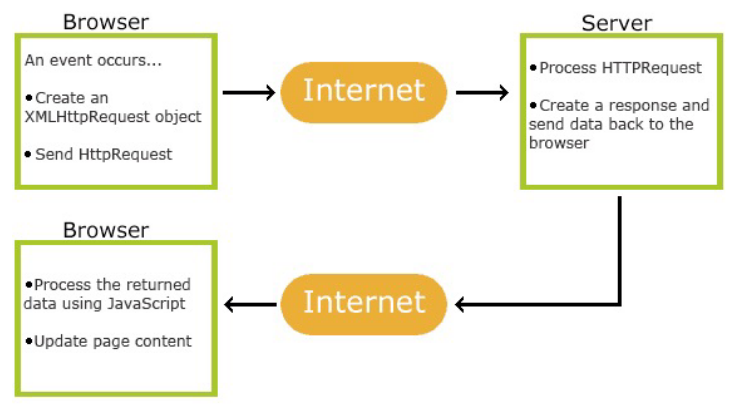
\includegraphics[width=0.65\textwidth]{figures/ajax.png}
	\caption{How AJAX Works}
	\label{fig:figures-ajax-png}
\end{figure}
\subsubsection{The XMLHttpRequest Object}
All modern browsers support the MLHttpRequestObject. It is this object that exchanges data behind the scenes. In javascript, this object can be created using
\begin{lstlisting}[language = Javascript , caption={XMLHttpRequest} , frame = trBL , firstnumber = last , escapeinside={(*@}{@*)}]
var xmlhttp = new XMLHttpRequest();
\end{lstlisting}
\subsubsection{Sending an XMLHttpRequest to the server}
To send a request to the server, we must first open the request
\begin{lstlisting}[language = Javascript , caption={open request} , frame = trBL , firstnumber = last , escapeinside={(*@}{@*)}]
xmlhttp.open("method","url","asynchronous");
\end{lstlisting}
\begin{itemize}
	\item Method - GET or POST to the URL
	\item URL - the resource we're interested in
	\item asynchronous - true/false
\end{itemize}
Secondly we use the send function
\begin{lstlisting}[language = Javascript , caption={Send function} , frame = trBL , firstnumber = last , escapeinside={(*@}{@*)}]
xmlhttp.send(); // for GET requests - url contains the query string
xmlhttp.send(string); // for POST requests
\end{lstlisting}
This sends request to the server
\subsubsection{Keeping track of the request}
When the request is sent, an onreadystatechange event is triggered every time the state changes. The readyState attribute holds the status of the event as an integer
\begin{enumerate}
	\item request not initialised
	\item server connection established
	\item request received
	\item processing request
	\item request finished and response complete	
\end{enumerate}
This event fires 5 times during the request for update.
\subsubsection{Processing the server response}
The response from the server can be accessed through the following attributes of XMLHttpRequest:
\begin{itemize}
	\item responseText - the response data as a string
	\item responseXML - the response data as XMl
\end{itemize}
The status of the request can be obtained through the $status$ property.
\subsubsection{Example}
Here we concern ourselves with readyState $4$ and a status of $200$ (OK).

\begin{lstlisting}[language = Javascript , caption={Asynchronous response} , frame = trBL , firstnumber = last , escapeinside={(*@}{@*)}]
xmlhttp.onreadystatechange=function() {
	if (xmlhttp.readyState==4 && xmlhttp.status==200) {
		document.getElementById("myDiv").innerHTMl=xmlhttp.responseText;
	}
}
\end{lstlisting}
\subsubsection{Handling JSON responses}
To create a javascript object from a JSON resposne, you can call the JSON.parse function. This function is included as part of all modern browsers. The complementary function is JSON.stringify which creates a JSON string from a javascript object. 
\subsubsection{What about jQuery}
Writing raw javascript to do these AJAX requests is quite longwinded. jQuery has some useful shorthand notation that we can use to make AJAX requests. jQuery has an ajax function that we can use to make requests a little more palletable. 
\begin{lstlisting}[language = Javascript , caption={AJAX in jQuery} , frame = trBL , firstnumber = last , escapeinside={(*@}{@*)}]
$.ajax({
	url = "/update"
	data: "{first_name: 'Andrew', last_name: 'Hague'}",
	success: updatePage();
});
\end{lstlisting}
The hash of options here includes
\begin{itemize}
	\item url
	\item data - the data to be passed to the server
	\item success - a callback function to execute when request completes
\end{itemize}
Ajax GET requests have a shorthand notation:
\begin{lstlisting}[language = Javascript , caption={GET Ajax jQuery} , frame = trBL , firstnumber = last , escapeinside={(*@}{@*)}]
$.get(url,sucess_callback);
//example
$.get("/status", function() {
	$('#status').html("OK");
});
\end{lstlisting}
And for post we use
\begin{lstlisting}[language = Javascript , caption={POST Ajax jQuery} , frame = trBL , firstnumber = last , escapeinside={(*@}{@*)}]
$.post(url,data,success_callback);
//example
$.post("/createTodo",
	{"title":"Buy Milk", "done":false},
	function(data) {
		var item = JSON.parse(data)
		var clone = $('#todos tbody tr').last().html();
		clone.children().first().html(item.title);
		$('#todos tbody').append(clone);
		}
);
\end{lstlisting}
\section{Web Development Hardware and Design}
\subsection{Usability and Accessibility}
Web developers must:
\begin{itemize}
	\item Work for an employer/client
	\item Be profitable
	\item Collaborate with non-programmers
	\item Work to deadlines
	\item Maintain a reputation
\end{itemize}
\subsubsection{Golden rules of Interaction design}
We must understand  the computer - its limitations, capacities, tools and platforms. Understand people - their psychology, social aspects and human error. And we need to understand human error - the err is to be human. \\
When an aspect of an interface is unclear, it is often blamed on user error and an additional paragraph is added to the help documentation or help screens. 
This means
\begin{tcolorbox}[colback=black!3!white,colframe=black!60!white,title=\begin{defn}User-centered design \label{User-centered design}\end{defn}]

\begin{enumerate}
	\item Put the user first
	\item Keep the user in the centre
	\item Remember the user at the end
\end{enumerate}
\end{tcolorbox}
\subsubsection{Software development lifecycle}
\begin{enumerate}
	\item Requirements capture
	\item Design
	\item Implementation
	\item Verification
	\item Maintenance
\end{enumerate}
\subsubsection{Requirements capture}
Elicitation - we need to work with stakeholder (product owner) and conduct interviews and questionnaires to ask users. Ethnography - we need to observe users and lastly consider scenarios and stories - start, normal activity, what goes wrong, what else can be happening and how it ends. 
\subsubsection{Types of requirements}
\textbf{Functional}\\
A service provided by the system and what it should not do\\
\textbf{Non functional}\\
Constraints on the functions and what can affect the whole system
\subsubsection{Specification}
What the system does, not how it does it. Describe using:
\begin{itemize}
	\item Natural language - easy for anyone
	\item Structure language - pseudocode
	\item Graphical notation - paper prototypes
	\item Design language - not for everyone
	\item Mathematical specification - very precise
\end{itemize}
Paper prototypes are quick and cheap to create and easy to change and iterate often. You are also able to get usability feedback from real users. 
\subsubsection{Usability}
Usability is made out of
\begin{itemize}
	\item Learnability - How easy is it for users to accomplish basic tasks the first time they encounter the design?
	\item Satisfaction - How pleasant is it to use the design?
	\item Efficiency - Once users have learned the design, how quickly can they perform tasks?
	\item Errors - How many errors do users make, how severe are these errors, and how easily can they recover from these errors
	\item Memorability - When users return to the design after a period of not using, how easily can they re-establish efficiency?
\end{itemize}
\subsubsection{Usability Concepts}
Visibility - can the user see how to use the website. The more visible the function, the easier it is for the user to use the function. The relationship between the position of control and what it does, is also vital to ease of use \\
Affordance - Related to visibility is the concept of affordance. It was used by Norman in 1992 as a technical term that refers to the properties of an object - what sort of operations can be done with a particular object\\
Perceived affordance - which of the buttons, for example, would denote a specific function?\\
Constraints - The concept of restraining the kind of user interaction that can take place at any one time. A common way of achieving this is to deactivate certain menu options by shading, thereby restricting their use. This prevents users from using it and thereby making mistakes.Constraints can also take of the form:
\begin{itemize}
	\item Physical - physical objects constrain the way they are used: DVD disk fits into DVD drive, not into USB port; Keyboard keys can usually only be pressed
	\item Logical - this refers to the users' understanding of the way world works. Making actions and their effect obvious allows users to deduce what happens next
	\item Cultural - Cultural conventions are learned conventions - colour red for danger or warnings is a typical western cultural convention. Most cultural constraints are arbitrary, but once learnt they are accepted as universal within that culture.
\end{itemize}
\subsubsection{Feedback}
Feedback is giving to the user information on what action has been done and what has been accomplished allowing the user to feel at ease and able to continue to operate successfully. Providing feedback of the right sort can aid visibility. Types of feedback include:
\begin{itemize}
	\item Visual - wait, an hourglass symbol on the interface
	\item Auditory - beep when a mistake is made by the user
	\item Tactile - touch of a keyboard, mouse
	\item Verbal - warnings given in sound, or welcome message
\end{itemize}
\subsubsection{Mapping}
Relations to the relationship between controls and their effects in the world. Good natural mapping examples include steering wheels, slider bars, cursor keys. Some poor mapping examples are taps and light switches - which switch switches which light?
\subsubsection{Consistency}
Similar operations should use similar elements for similar tasks. For example, cut and paste are always in the edit menu. File menu top left, help in top right in windows.
\subsubsection{Usability Heuristics}
\begin{enumerate}
	\item Visibility of system status - keep users informed of status by providing appropriate feedback (visual, auditory or tactile as appropriate)
	\item Match between system and real world - Use user's language rather than system terms
	\item User control and freedom - Provide "escape routes for users"
	\item Consistency and standards - avoid making users wonder if different words mean the same thing
	\item Error prevention - prevent users from making errors in the first place where possible. Think about user's existing model and how it can be utilised
	\item Recognition rather than recall - make objects, actions and options visible
	\item Flexibility and efficiency of use - provide accelerators that allow experts to do things faster
	\item Aesthetic and minimalist design - avoid using information that is irrelevant or rarely needed
	\item Help users recognise, diagnose and recover from error - use plain language to describe the nature of error and its solution. Be informative and non-technical, indicate something has gone wrong and provide potential solution
	\item Help and documentation - provide information that is easily searched and provides help with concrete solutions.
\end{enumerate}
	\subsubsection{Accessibility}
	The inclusive practice of making websites useable by people of all abilities. It is a legal requirement (Equality Act 2010).
	\begin{itemize}
		\item Meet level AA of the web content accessibility guidelines (WCAG 2.1)
		\item Otherwise; you could be sued for discrimination
	\end{itemize}
	At a basic level, a site is coded semantically using HTML, has text equivalents for images and meaningful link names.
	\subsubsection{Accessibility Needs }
	\begin{itemize}
		\item Visual - blindness, poor vision, colour blindness
		\item Motor - difficulty in using hands (tremors, muscle slowness, loss of fine muscle control)
		\item Auditory - deafness / hearing impairments
		\item Seizures - epilepsy brought on by flashing lights
		\item Cognitive - developmental disabilities, learning difficulties, memory problems and attention
	\end{itemize}
	Some ways of making accessible is by increasing image size, making critical information bold and links underlined, making clickable areas large
	\subsubsection{Assistive technologies}
	\begin{itemize}
		\item Screen reading software - reads the content of the screen to the user using synthesised speech.
		\item Braille terminals output text as braille
		\item Screen magnification
		\item Speech recognition
		\item Large trackballs
	\end{itemize}
	\subsubsection{WCAG 2.1}
	Web content accessibility guidelines (WCAG) are published by the Web Accessibility Initiative. WCAG 2.0 was publishedi n 2008 and became an ISO standard in 2012. WCAG 2.1 was published in 2018. It contains four principles:
	\begin{enumerate}
		\item Perceivable - information and user interface components must be presentable to users in ways they can perceive
		\item Operable - user interface components and navigation must be operable
		\item Understandable - information and the operation of user interface must be understandable
		\item Robust - content must be robust enough that it can be interpreted reliably by a wide variety of user agents, including assistive technologies
	\end{enumerate}
\subsection{Evaluation and Testing}
Evaluation is the process of gathering data about the usability of a design, the characteristics of the user and the activities the user will do next. The environment and the context where the evaluation will take place and the nature of the artefact being examined. 
\subsubsection{Formative vs Summative Evaluation}
\begin{itemize}
	\item Formative evaluation - evaluation of an existing product, predictive evaluation, feedback from evaluation
	\item Summative evaluation - evaluation at the completion of a product
\end{itemize}
\subsubsection{Measuring usability}
Examples include ratio of successes to failures, time to complete task, number of errors user makes and number of times the user expresses frustration or satisfaction. 
\subsection{Web architecture and performance}
\subsubsection{Software Stack}
Even our simple application uses several software components. Software components that work together are referred to as a stack. For example, web server (aoache), Applications (python/flask) and database (SQLite). There is also three tier architecture involved:
\begin{figure}[H]
	\centering
	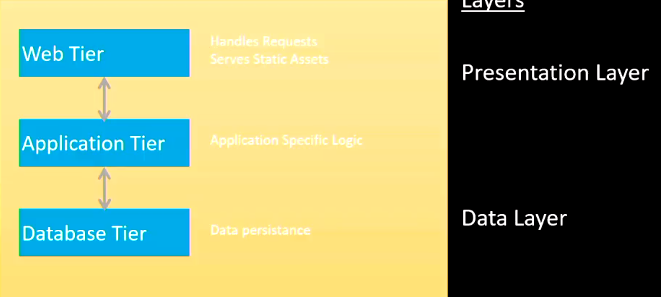
\includegraphics[width=0.6\textwidth]{figures/layer.png}
	\caption{Three tier architecture}
	\label{fig:figures-layer-png}
\end{figure}
\subsubsection{Servers}
When a system ran out of capacity, you bought a bigger system. This is known as vertical scaling/scaling up. This is still practical to a certain degree. Even 1U servers can support huge quantities of RAM and have large disks. There are 42 units in a standard rack. We do not really buy servers anymore though. The advantages are:
\begin{itemize}
	\item Can buy minimally specified system now and upgrade RAM or add disks as you grow
	\item Minimizes your capital expenditure on hardware
\end{itemize}
The disadvantages are:
\begin{itemize}
	\item The whole machine must be replaced when its total capacity is exceeded.
	\item Upgrading/replacing the machine leads to downtime
\end{itemize}
A more modern approach to this is the database system is placed on a different server.
\begin{itemize}
	\item RDBMS work best when they can cache large quantities of data in RAM
	\item This does however increase the latency of every request as they must now be sent over the network
\end{itemize}
Multiple copies of our web server and application are allocated to different servers
\begin{itemize}
	\item These can be reasonably low capacity servers
\end{itemize}
And we have then a load balancer which redirects the user to a lowest traffic server. The algorithms can be used to balance the requests:
\begin{itemize}
	\item Round robin - requests are sent to each server in turn
	\item Weighted round robin - requests are sent to each server in turn, as determined b an associated weight for each server
	\item Least active server - requests are sent to most lightly loaded server
\end{itemize}
However, the are disadvantages:
\begin{itemize}
	\item More server maintenance is required
	\item Requires more server expenditure
\end{itemize}
the advantage is that
\begin{itemize}
	\item Relatively cheap to add capacity - just add a server to load balancer
	\item Failure of web servers can easily be handled
\end{itemize}
\subsubsection{Cloud based infrastructure}
Cloud based infrastructure is rather:
\begin{itemize}
	\item Cheap, reduces capital expenditure i.e., no need to pay for anything upfront as it scales as you use it
	\item Easily scaling - we can add resources as required, so no need to worry about capacity management
\end{itemize}
\subsubsection{Additional software components}
Caches
\begin{itemize}
	\item Results of heavy computation maybe cached (stored)
	\item This means that computation does not need to have to be carried out again
	\item For example, memcached or varnish.
\end{itemize}
Message queues
\begin{itemize}
	\item Some applications have long running tasks
	\item Waiting for this to be done would take a significant amount of time
	\item Applications can drop messages into a queue, which are then processed by software which listens to the queue
\end{itemize}
\subsubsection{Performance}
Performance can be measured using:
\begin{itemize}
	\item End to end response time - the time taken from issuing a request to it being returned
	\item Site response time - this measures the time taken for the server to process a request
	\item Request throughput - the number of requests processed by a server per second
\end{itemize}
Note that response times do not necessarily increase linearly, therefore bulletpoint 1 and bulletpoint 2 are separate. Failure to have good performance an cause in page abandonment, good first impressions and loser users results in lost revenue. Now, which one to use? \\
We can test for concurrent users, end to end response time or throughput. Furthermore, we can measure end-to-end response time is sending a lot of request to the server and measure the time taken. The response time is an average of these. This needs to be done for each request type with appropriate tools. \\ 
Throughput can be measured by primarily concerning with how many requests your system can service per unit time. Need to consider the range of request types in your application. Each request will represent a different proportion of application actions. We'd usually send a large number of requests, requests should be executed at varying levels of concurrency to investigate the throughput of the system and plot the results and view the performance curve. \\
Concurrent users can be tested by considering what a typical user does in a session, how many times they visit each page and what is a reasonable think time, where think time is time taken by a user to process information. An exponentially distributed think-with a mean of 7 seconds is common. 
\subsubsection{Typical application growth path}
\begin{enumerate}
	\item Start small - single server
	\item Add in a dedicated server
	\item Add in a second application server and load balance
	\item Scale as required
\end{enumerate}
\section{Supporting Mobile}
There has been a vast increase in the amount of mobile web traffic over the past few years. This is largely down to our handheld, IoT, smart home devices. The widespread adoption of these causes significant issues for web developers such as
\begin{itemize}
	\item Small screen sizes
	\item Touch based interactions
	\item Headless web services
\end{itemize}
There are two main techniques which are
\begin{itemize}
	\item Responsive web design
	\item Creation of separate pages for mobile platforms and web services
\end{itemize}
\subsection{Responsive web design}
For responsive web design, we focus on interactive web pages. The central notion for this is that one design should work across all designs e.g., desktops, tablets and mobile phones. This works by utilising an advanced feature of CSS3 called $media$ queries. You can use these to asses the capabilities of the device:
\begin{itemize}
	\item Height/width of browser window
	\item Height/width of device
	\item Orientation - landscape/portrait
	\item Resolution
\end{itemize}
You can use the media queries in the CSS file directly or we can add links to different CSS files in the head element. We simply add a section which is delimited by an $@media$ tag. Max-device-width can also be used for a browser screen which doesn't normally change size.
\begin{lstlisting}[language = CSS , caption={Media queries} , frame = trBL , firstnumber = last , escapeinside={(*@}{@*)}]
@media only scree and (max-width:480px) {
	div#wrapper {
		width: 400px;
	}
	div#header {
		background-image: url(media-quieries-phone.jpg);
		height: 93px;
		position: relative;
	}
	div#header h1 {
		font-size: 140%;
	}
	#content {
		float: none;
		width: 100%;
	}
	#navigation {
		float: none;
		width: auto;
	}
}
\end{lstlisting}
We do this as it saves a lot of hassle rewriting whole pages. You can simply use your existing content and it will be laid out in the best format for the device. 
\subsection{CSS Layout and Flexbox}
We can combine with media query for responsive layout. Flexbox can be found in flexbox.help link website. 
\subsection{Creating a separate mobile layout}
You might choose to have an entirely separate site for mobile content. This was previously a very common approach. You can do a redirect based on the browser's UserAgent which is sent in the header. User agent is accessed by
\begin{lstlisting}[language = Python , caption={User Agent} , frame = trBL , firstnumber = last , escapeinside={(*@}{@*)}]
request.user_agent
\end{lstlisting}
IT is sent as a part of the HTTP request and contains more information than one would think. We can access the user agent in python with the code above. Use this information to build a different user experience. You could then check it against known value for mobile devices. \\
However, there is already a library in flask which can help use recognise the device being used instead of accessing it from request.user$\_$agent.string which is flask-mobility.
\begin{lstlisting}[language = Python , caption={Flask-mobility} , frame = trBL , firstnumber = last , escapeinside={(*@}{@*)}]
from flask_mobility import Mobility
from flask_mobilidy.decorators import mobile_template

@app.route('/mobile')
@mobile_template('{mobile/}index.html')
def mob(template):
	return render_template(template)
\end{lstlisting}
\subsubsection{Pros}
\begin{itemize}
	\item Easy to create separate fixed width views
	\item Hard to cater for all sizes of screen
\end{itemize}
\subsubsection{Cons}
\begin{itemize}
	\item May not work if new user agents are created
	\item May be lots of work to double the pages
\end{itemize}
\section{Being a web developer}
\subsection{Testing}
There are various types of testing:
\begin{itemize}
	\item Functional testing
	\item Usability testing
	\item Compatibility testing
	\item Performance testing
	\item Security testing
\end{itemize}
\subsubsection{Functional Testing}
\begin{itemize}
	\item Test all pages for errors
	\item Test all forms, check the results of the operation and check your validations are working appropriately. 
\end{itemize}
\subsubsection{Usability Testing}
\begin{itemize}
	\item Is navigating your application easy?
	\item Is the content correct?
	\item Link to help docs?
	\item Have you considered accessibility
\end{itemize}
\subsubsection{Compatibility Testing}
Browsers - we've only been really testing with Chrome and Firefox, what about edge, safari and opera? Or mobile devices, tablets (MS surface). What happens if a user is using an unsupported browser?
\subsubsection{Performance Testing}
How fast is your application? Can you optimise your apps such as caching data/assets, more efficient queries
\subsubsection{Security Testing}
is your application vulnerable to SQL injection attacks? Especially important if your chosen framework uses raw SQL. What is your update policy and what about your software stack? 
\subsubsection{When to run tests}
It is recommended that the tests are ran frequently. Tests are ran manually after implementing every feature. Continuous Integration (CI), our tests run automatically when we check code into central repository. 
\end{document}


